\documentclass[aspectratio=169, pdf, 8pt, unicode]{beamer}
\usepackage[american,russian]{babel}
\usepackage[default]{sourcesanspro}
\usepackage{float}
\usepackage{graphicx}
\usepackage{pgfplotstable}
\usepackage{caption}
\usepackage{amsmath}
\usepackage{amssymb}
\usepackage{graphicx}
\usepackage{tikz}
\usetikzlibrary{automata, positioning, arrows, chains, fit, shapes}
\usepackage{tikzscale}
\usepackage{setspace}
\usepackage[outputdir=aux]{minted}

\DeclareCaptionLabelFormat{gostfigure}{Рисунок #2}
\captionsetup[table]{labelsep=endash,justification=justified,singlelinecheck=false,font=normalsize,skip=0pt} 
\captionsetup[figure]{labelformat=gostfigure,labelsep=endash,justification=centering,singlelinecheck=false,font=normalsize} 
\pgfplotsset{compat=1.9}

\mode<presentation> {
\usetheme{Madrid}
}

\newcounter{defCnt}
\newcounter{thmCnt}

\setbeamerfont{institute}{size=\normalsize}
\setbeamertemplate{itemize/enumerate body begin}{\large}
\setbeamertemplate{itemize/enumerate subbody begin}{\tiny}

\title[Теория и практика многопоточного программирования]{Теория и практика многопоточного программирования\\ \vspace{0.5cm}Лекция 7}

\author{Неганов Алексей}

\institute[МФТИ]{
    Московский физико-технический институт (национальный исследовательский университет)\\
    Кафедра теоретической и прикладной информатики\\
}

\date{Москва 2020}

\setbeamertemplate{caption}[numbered]

\begin{document}

\begin{frame}
\titlepage
\end{frame}

\begin{frame}[fragile]
\frametitle{Соисполняющиеся объекты}
\begin{figure}[H]
\centering
\begin{minipage}{0.8\textwidth}
\begin{minted}[linenos]{C++}
template <class T> 
class waitFreeQueue {
    atomic_int head, tail;
    int len;
    T *items;

public:
    waitFreeQueue(int cap): head(0), tail(0), len(cap) {
        items = new T[cap];
    }
    void enq(T x) {
        items[tail % len] = x;
        tail++;
    }
    T deq() {
        if (tail == head)
            throw;
        T x = items[head % len];
        head++;
        return x;
    }
};
\end{minted}
\end{minipage}
\end{figure}
\end{frame}

\begin{frame}
\frametitle{Соисполняющиеся объекты}
\begin{itemize}
\setlength\itemsep{2em}
    \item \textbf{Bызов метода} --- интервал между событиями \texttt{invocation} и \texttt{response}
    \item \textbf{Precondition} --- состояние объекта до события \texttt{invocation}
    \item \textbf{Postcondition} --- состояние объекта после события \texttt{response}
    \item \textbf{Side effect} --- изменение состояния объекта при вызове метода
\end{itemize}
\end{frame}

\begin{frame}
\frametitle{Quiescent consistency}
\stepcounter{defCnt}
\begin{block}{Определение \arabic{defCnt}}
    Объект называется \textbf{покоящимся} \textit{(quiescent),} если в данный момент времени нет ожидающих вызовов методов объекта. 
\end{block}
\begin{exampleblock}{Принцип 1}
    Вызовы методов должны происходить <<по одному за раз>> и последовательно.
\end{exampleblock}
\begin{exampleblock}{Принцип 2}
    Вызовы методов, разделённые периодами покоя, должны давать результат в том порядке, в котором методы вызываются \textbf{в реальном времени}.
\end{exampleblock}
\stepcounter{defCnt}
\begin{block}{Определение \arabic{defCnt}}
    Вызовы методов, удовлетворяющие одновременно принципам 1 и 2, называются \textbf{согласованными по периодам покоя}
    \textit{(quiescently consistent)}.
\end{block}
\end{frame}

\begin{frame}[fragile]
\frametitle{Quiescent consistency}
\stepcounter{defCnt}
\begin{block}{Определение \arabic{defCnt}}
    Метод называется \textbf{тотальным} \textit{(total),} если он определён для каждого состояния объекта,
    и \textbf{частичным} \textit{(partial)} в противном случае.
\end{block}
\stepcounter{defCnt}
\stepcounter{thmCnt}
\begin{block}{Теорема \arabic{thmCnt} (о неблокируемости QC)}
    Для любого соисполнения любых незавершённых вызовов тотальных методов существуют события завершения вызова \texttt{(response)},
    согласованные по периодам покоя.
\end{block}
Это значит, что если вызов начался для тотального метода, он не должен дожидаться завершения любого другого незаконченного вызова.
\begin{block}{Определение \arabic{defCnt}}
    Свойство корректности $P$ называется \textbf{композиционным} для системы объектов, если из того, что каждый объект системы
    обладает $P$, следует, что и система в целом обладает $P$.
\end{block}
\stepcounter{thmCnt}
\begin{block}{Теорема \arabic{thmCnt}}
    Свойство согласованности по периодам покоя является композиционным.
\end{block}
\end{frame}

\begin{frame}[fragile]
\frametitle{Sequential consistency}
\begin{exampleblock}{Принцип 3}
    Результаты вызовов методов должны получаться в том порядке, который \textbf{определён программой}.
\end{exampleblock}
\stepcounter{defCnt}
\begin{block}{Определение \arabic{defCnt}}
    Вызовы методов, удовлетворяющие одновременно принципам 1 и 3, называются \textbf{упорядоченно согласованными}
    \textit{(sequentially consistent)}.
\end{block}
\begin{block}{Замечание}
    Из упорядоченной согласованности не следует согласованность по периодам покоя, как и наоборот.
\end{block}
\stepcounter{thmCnt}
\begin{block}{Теорема \arabic{thmCnt}}
    Свойство упорядоченной согласованности НЕ является композиционным.
\end{block}
\end{frame}

\begin{frame}[fragile]
\frametitle{Sequential consistency}
\begin{figure}[H]
\centering
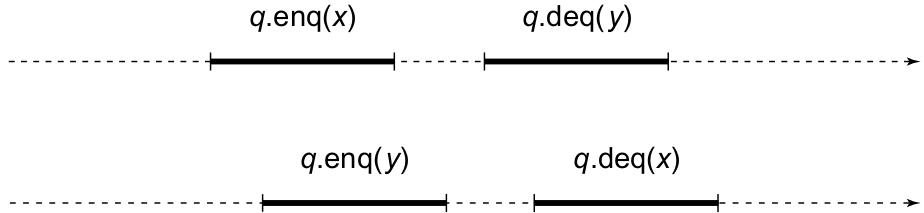
\includegraphics[width=0.7\textwidth]{fig/sequential_consistency_1.png}
\\
\bigskip
Назовите упорядоченно согласованный порядок исполнения вызовов. Является ли он единственным?
\end{figure}
\begin{figure}[H]
\centering
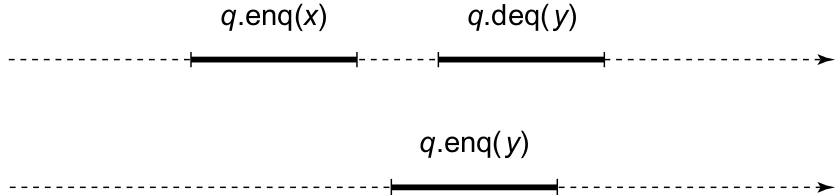
\includegraphics[width=0.7\textwidth]{fig/sequential_consistency_2.png}
\\
\bigskip
Можно ли назвать такое исполнение упорядоченно согласованным?
\end{figure}
\end{frame}

\begin{frame}[fragile]
\frametitle{Linearizability}
\begin{exampleblock}{Принцип 4}
    Изменения данных, как результат применения метода, имеют место непосредственно между событиями его вызова и завершения.
\end{exampleblock}
\stepcounter{defCnt}
\begin{block}{Определение \arabic{defCnt}}
    Вызовы методов, удовлетворяющие одновременно принципам 1 и 4, называются \textbf{линеаризуемыми}
    \textit{(linearizable)}.
\end{block}
\begin{block}{Замечание}
    Из линеаризуемости очевидно следует упорядоченная согласованность, обратное неверно.
\end{block}
\stepcounter{defCnt}
\begin{block}{Определение \arabic{defCnt}}
    \textbf{Точка линеаризации} --- то место, где изменения данных, явившиеся следствиям изменения метода, имеют эффект.
\end{block}

Как будет показано далее, свойство линеаризуемости является неблокирующим и композиционным.
\end{frame}

\begin{frame}
\frametitle{Понятие <<истории>>}

\stepcounter{defCnt}
\begin{block}{Определение \arabic{defCnt}}
    \textbf{История} $H$ представляет собой конечную последовательность событий типа \texttt{invocation} и \texttt{response} для методов.
    Подпоследовательность $S$ событий из $H$ называется \textbf{подысторией}.
\end{block}

\stepcounter{defCnt}
\begin{block}{Определение \arabic{defCnt}}
    Будем называть событие \texttt{response} \textbf{соответствующим} событию \texttt{invocation}, если они относятся к тому же объекту и
    потоку исполнения. \textbf{Вызов метода} в истории $H$ есть пара событий \texttt{invocation} и соответствующее ему \texttt{response};
    если же такого события не существует, то вызов метода называется \textbf{ожидающим} \textit{(pending)}.
\end{block}

\stepcounter{defCnt}
\begin{block}{Определение \arabic{defCnt}}
    \textbf{Расширением} истории $H$ будем называть историю $H^{\prime}$, содержащую $H$ и 0 или более событий типа \texttt{response}
    для ожидающих вызовов.
\end{block}

\stepcounter{defCnt}
\begin{block}{Определение \arabic{defCnt}}
    \textbf{Завершённой} историей для истории $H$ будем называть историю $\mathrm{complete}(H)$, содержащую подпоследовательность пар всех
    соответствующих событий $H$, без ожидающих вызовов.
\end{block}

\end{frame}

\begin{frame}
\frametitle{Понятие <<истории>>}

\stepcounter{defCnt}
\begin{block}{Определение \arabic{defCnt}}
    Историю $H$ будем называть \textbf{упорядоченной} \textit{(serialized)}, если первое событие $H$ есть \texttt{invocation}, и каждое событие
    \texttt{invocation}, возможно, за исключением последнего, имеет непосредственно следующее за ним событие \texttt{response}.
\end{block}

Начало вызова метода $m$ объекта $x$ c последовательностью аргументов $a^*$ в потоке $A$ обозначим $\langle x.m(a^*)A \rangle$.
Аналогично, $\langle x \colon t(r^*)A \rangle$ представляет собой событие конца вызова, где $t$ ---
обозначение для успешного завершения метода или имя ошибки
(исключения), а $r^*$ --- последовательность выходных значений.

\textbf{Подыстория потока} $H|A$ есть подпоследовательность всех событий $H$, в которых поток есть $A$. Аналогично определяется
подыстория объекта $H|x$. Историю $H$ такую, что для каждого потока $A$ подыстория $H|A$ упорядочена, называют \textbf{правильной}
\textit{(well formed)}.

Обозначим факт предшествования события \texttt{response} метода $m_0$ событию \texttt{invocation} метода $m_1$ как $m_0 \to_H m_1$.
Для подыстории $H|x$ будем писать $m_0 \to_x m_1$.

\stepcounter{defCnt}
\begin{block}{Определение \arabic{defCnt}}
    Упорядоченную историю $H$ будем называть \textbf{легальной} \textit{(legal)}, если для каждого объекта его подыстория легальна
    для объекта.
\end{block}

\end{frame}

\begin{frame}
\frametitle{Линеаризация истории}

\stepcounter{defCnt}
\begin{block}{Определение \arabic{defCnt}}
    История $H$ является \textbf{линеаризуемой}, если для её расширения $H^{\prime}$ существует легальная упорядоченная история $S$
    такая, что:
    \begin{equation}
    \begin{aligned}
        & \mathrm{complete}(H) = S;\\
        & \text{если } m_0 \to_H m_1, \text{то } m_0 \to_S m_1.\\
    \end{aligned}
    \end{equation}
\end{block}

\stepcounter{thmCnt}
\begin{block}{Теорема \arabic{thmCnt} (композиционность линеаризуемости)}
    Для того, чтобы $H$ была линеаризуемой, необходимо и достаточно, чтобы для каждого объекта $x$ подыстория $H|x$ была линеаризуемой.
\end{block}

Доказательство достаточности: индукция по количеству вызовов в $H^{\prime}$.

\stepcounter{thmCnt}
\begin{block}{Теорема \arabic{thmCnt} (неблокируемость линеаризации)}
    Если $\langle x \: \mathrm{inv} \: P \rangle$ есть ожидающий вызов тотального метода в линеаризуемой истории $H$, то существует событие конца вызова
    $\langle x \: \mathrm{res} \: P \rangle$, такое, что $H \langle \mathrm{res} \: P \rangle$ --- линеаризуемая история.
\end{block}

\end{frame}

\begin{frame}
\frametitle{Упражнения}
Пусть $r$ --- операция чтения из регистра чтения-записи, а $w$ --- операция записи.
\begin{itemize}
\setlength\itemsep{2em}
\item Пусть $H|A = \langle x.w(1)A \rangle \langle x.r(1)A \rangle$, $H|B = x.w(2)B$, причём записи соисполняемы, а чтение и запись -- нет.
    Является ли исполнение линеаризуемым?
    \item Является ли исполнение с историей $H = \langle x.w(1)A \rangle \langle x.r(2)B \rangle$ линеаризуемым, если операции разделены периодом покоя?
    \item Пусть $H|A = \langle x.w(0)A \rangle \langle x.r(1)A \rangle$, $H|B = \langle x.w(1)B \rangle$. Является ли исполнение упорядоченно согласованным?
    \item Пусть $H|A = \langle x.w(1)A \rangle \langle x.r(3)A \rangle \langle x.w(3)A \rangle$, причём между первой и второй операцией имеется
        период покоя; $H|B = \langle x.w(2)B \rangle$, причём эта операция соисполняема с последними двумя операциями потока $A$.
        Будет ли такое исполнение согласованным по периодам покоя?

\end{itemize}
\end{frame}

\end{document}
